\documentclass[10pt,a4paper]{article}
\usepackage[utf8]{inputenc}
\usepackage[T1]{fontenc}
\usepackage{polski}
\usepackage{lmodern}
\usepackage[a4paper,margin=2.0cm]{geometry}
\usepackage{amsmath,amssymb}
\usepackage{graphicx}
\usepackage{booktabs,tabularx,array}
\usepackage{caption}
\usepackage{microtype}
\emergencystretch=2em
\usepackage{xcolor}
\usepackage[colorlinks=true,linkcolor=blue,urlcolor=blue]{hyperref}
\captionsetup{font=small,labelfont=bf}
\setlength{\parskip}{3pt}
\setlength{\parindent}{0pt}
% generated by analysis.py - do not edit
\newcommand{\NCzero}{35.0}
\newcommand{\NDNazero}{1426}
\newcommand{\NDNazeroErr}{58}
\newcommand{\NEKnowles}{-0.319}
\newcommand{\NFpval}{0.00}
\newcommand{\NFpvalOnek}{0.009}
\newcommand{\NFstat}{9.41}
\newcommand{\NFstatOnek}{2.62}
\newcommand{\NGcalAtCzero}{-52.13}
\newcommand{\NGfromKzero}{-52.77}
\newcommand{\NISEglycerol}{6}
\newcommand{\NKzero}{1.76}
\newcommand{\NMUXKCL}{0.035}
\newcommand{\NPKnowles}{+0.396}
\newcommand{\NSKhighc}{1.14}
\newcommand{\NSKlocal}{3.47}
\newcommand{\NSKlocalErr}{0.10}
\newcommand{\NSKmodel}{2.95}
\newcommand{\NSKmodelErr}{0.05}
\newcommand{\NSdosyA}{+0.188}
\newcommand{\NSdosyB}{+0.098}
\newcommand{\NSdosyC}{+0.061}
\newcommand{\Natfourzeroa}{+11.3}
\newcommand{\Natfourzerob}{+7.7}
\newcommand{\Natfourzeroc}{+3.7}
\newcommand{\Natfourzerodone}{+2.3}
\newcommand{\Natfourzerodtwo}{+1.6}
\newcommand{\Natfourzeroe}{-4.2}
\newcommand{\NbOneCV}{19}
\newcommand{\NbOneCVOnek}{10}
\newcommand{\NbOneChi}{3.3}
\newcommand{\NbOneMean}{-0.234}
\newcommand{\NbOneMeanErr}{0.015}
\newcommand{\NbTwoCV}{5}
\newcommand{\NbTwoChi}{0.2}
\newcommand{\NbTwoMean}{+21.3}
\newcommand{\NbTwoMeanErr}{1.2}
\newcommand{\NbnCodeEG}{0.43}
\newcommand{\NbnCodeEGErr}{0.07}
\newcommand{\NbnCodePEGtwo}{0.80}
\newcommand{\NbnCodePEGtwoErr}{0.05}
\newcommand{\NbnSelfEG}{-0.034}
\newcommand{\NbnSelfEGErr}{0.154}
\newcommand{\NbnSelfPEGtwo}{0.034}
\newcommand{\NbnSelfPEGtwoErr}{0.121}
\newcommand{\NbnSelfQuadEG}{-0.066}
\newcommand{\NbnSelfQuadPEGtwo}{-0.002}
\newcommand{\NbnUpperEG}{0.27}
\newcommand{\NbnUpperPEGtwo}{0.28}
\newcommand{\NbroSone}{-0.916}
\newcommand{\NbroSoneErr}{0.225}
\newcommand{\NbroStwo}{+0.100}
\newcommand{\NbroStwoErr}{0.007}
\newcommand{\NbroSixSone}{-0.260}
\newcommand{\NbroSixSoneErr}{0.021}
\newcommand{\NbroSixStwo}{+0.185}
\newcommand{\NbroSixStwoErr}{0.021}
\newcommand{\NbroXsMax}{1.3}
\newcommand{\NbroXsMin}{-1.6}
\newcommand{\NcEGforty}{6.87}
\newcommand{\NcEqEG}{5.5}
\newcommand{\NchiFreeTot}{66}
\newcommand{\NchiJointRed}{26.5}
\newcommand{\NchiQuadTot}{407}
\newcommand{\NchiSepRed}{10.0}
\newcommand{\NchiSixTot}{435}
\newcommand{\NcollconstAllAlpha}{-0.95}
\newcommand{\NcollconstAllRtwo}{0.87}
\newcommand{\NcollconstPEGAlpha}{-0.94}
\newcommand{\NcollconstPEGRtwo}{0.86}
\newcommand{\NcollrealAlpha}{-0.75}
\newcommand{\NcollrealRtwo}{0.90}
\newcommand{\NcurvObsSigma}{14.5}
\newcommand{\Ncurva}{-35.4}
\newcommand{\Ncurvb}{-32.0}
\newcommand{\Ncurvc}{-15.7}
\newcommand{\Ncurvobs}{+93.2}
\newcommand{\NddGEGforty}{14.7}
\newcommand{\NddGEGfortyErr}{0.5}
\newcommand{\NddGobsFortyPEGthirtyfive}{-0.3}
\newcommand{\NegExplCode}{5.4}
\newcommand{\NegExplFracCode}{37}
\newcommand{\NegExplFracKappa}{20}
\newcommand{\NegExplFracUpper}{28}
\newcommand{\NegExplKappa}{2.9}
\newcommand{\NegExplUpper}{4.1}
\newcommand{\NfracMaxa}{77}
\newcommand{\NfracMaxb}{45}
\newcommand{\NfracMaxc}{22}
\newcommand{\NfracMaxdone}{15}
\newcommand{\NfracMaxdtwo}{11}
\newcommand{\NfracMaxe}{-31}
\newcommand{\NfracMeana}{69}
\newcommand{\NfracMeanb}{41}
\newcommand{\NfracMeanc}{20}
\newcommand{\NfracMeandone}{14}
\newcommand{\NfracMeandtwo}{10}
\newcommand{\NfracMeane}{-36}
\newcommand{\NfracMina}{62}
\newcommand{\NfracMinb}{37}
\newcommand{\NfracMinc}{18}
\newcommand{\NfracMindone}{12}
\newcommand{\NfracMindtwo}{9}
\newcommand{\NfracMine}{-41}
\newcommand{\NiseSlopeBuf}{52.9}
\newcommand{\NiseSlopeEG}{53.3}
\newcommand{\NkappaCode}{0.168}
\newcommand{\NknASAI}{82.5}
\newcommand{\NknAlphaI}{-2.21}
\newcommand{\NknChiInf}{0.45}
\newcommand{\NknDASA}{2006}
\newcommand{\NknEG}{0.34}
\newcommand{\NknEV}{0.309}
\newcommand{\NknHigh}{-0.156}
\newcommand{\NknHighErr}{0.020}
\newcommand{\NknHighQuad}{-0.25}
\newcommand{\NknMuMann}{-0.0015}
\newcommand{\NknMuMannErr}{0.014}
\newcommand{\NknMuOne}{0.0378}
\newcommand{\NknMuSorb}{0.0082}
\newcommand{\NknMuSorbErr}{0.013}
\newcommand{\NknMuTwo}{0.0324}
\newcommand{\NknMuXyl}{0.0019}
\newcommand{\NknMuXylErr}{0.007}
\newcommand{\NknPEGtwo}{0.21}
\newcommand{\NknXrev}{6}
\newcommand{\NmEG}{+0.319}
\newcommand{\NmEGErr}{0.124}
\newcommand{\NmPEGonetwok}{-0.348}
\newcommand{\NmPEGonetwokErr}{0.176}
\newcommand{\NmPEGonek}{-0.324}
\newcommand{\NmPEGonekErr}{0.178}
\newcommand{\NmPEGonepfivek}{-0.297}
\newcommand{\NmPEGonepfivekErr}{0.169}
\newcommand{\NmPEGtwozerozero}{+0.008}
\newcommand{\NmPEGtwozerozeroErr}{0.162}
\newcommand{\NmPEGtwozerok}{-0.365}
\newcommand{\NmPEGtwozerokErr}{0.185}
\newcommand{\NmPEGthreefivek}{-0.348}
\newcommand{\NmPEGthreefivekErr}{0.166}
\newcommand{\NmPEGthreek}{-0.381}
\newcommand{\NmPEGthreekErr}{0.173}
\newcommand{\NmPEGfourzerozero}{-0.027}
\newcommand{\NmPEGfourzerozeroErr}{0.141}
\newcommand{\NmPEGsixzerozero}{-0.140}
\newcommand{\NmPEGsixzerozeroErr}{0.166}
\newcommand{\NmPEGsixk}{-0.367}
\newcommand{\NmPEGsixkErr}{0.168}
\newcommand{\NmPEGtwoFull}{+0.184}
\newcommand{\NmPEGtwoFullErr}{0.045}
\newcommand{\NmeanTwenty}{-4.2}
\newcommand{\NnBroTot}{50}
\newcommand{\NnSIbeyond}{5}
\newcommand{\NnullChi}{0.1}
\newcommand{\NnullE}{-0.485}
\newcommand{\NnullEErr}{0.086}
\newcommand{\NnullMaxRes}{0.8}
\newcommand{\NnullNh}{8}
\newcommand{\NnullNhErr}{3}
\newcommand{\NnullP}{+0.290}
\newcommand{\NnullPErr}{0.124}
\newcommand{\NonePlusEps}{0.92}
\newcommand{\NplateauKnowlesPred}{-0.140}
\newcommand{\NpredChi}{2.3}
\newcommand{\NratioMaxEG}{1.05}
\newcommand{\NratioMaxPEGtwo}{1.03}
\newcommand{\NratioMeanEG}{0.999}
\newcommand{\NratioMeanEGErr}{0.023}
\newcommand{\NratioMeanPEGtwo}{0.990}
\newcommand{\NratioMeanPEGtwoErr}{0.019}
\newcommand{\NratioMinEG}{0.94}
\newcommand{\NratioMinPEGtwo}{0.95}
\newcommand{\NreqFullConsBn}{5.79}
\newcommand{\NreqFullConsFactor}{40.8}
\newcommand{\NreqFullConsFrac}{98}
\newcommand{\NreqFullConsmV}{95}
\newcommand{\NreqFullManBn}{0.78}
\newcommand{\NreqFullManFactor}{6.4}
\newcommand{\NreqFullManFrac}{84}
\newcommand{\NreqFullManmV}{48}
\newcommand{\NreqLinConsBn}{4.34}
\newcommand{\NreqLinConsFactor}{30.9}
\newcommand{\NreqLinConsFrac}{97}
\newcommand{\NreqLinConsmV}{88}
\newcommand{\NreqLinManBn}{0.66}
\newcommand{\NreqLinManFactor}{5.6}
\newcommand{\NreqLinManFrac}{82}
\newcommand{\NreqLinManmV}{44}
\newcommand{\NrestMean}{-9.3}
\newcommand{\NrestSD}{2.3}
\newcommand{\NsaltChi}{0.1}
\newcommand{\NsaltS}{-0.167}
\newcommand{\NsaltSErr}{0.086}
\newcommand{\NsddGzero}{0.44}
\newcommand{\NspreadTwenty}{2.0}
\newcommand{\NswingPEGonetwok}{6.6}
\newcommand{\NswingPEGonetwokErr}{1.9}
\newcommand{\NswingPEGonek}{8.5}
\newcommand{\NswingPEGonekErr}{2.7}
\newcommand{\NswingPEGonepfivek}{8.0}
\newcommand{\NswingPEGonepfivekErr}{0.8}
\newcommand{\NswingPEGtwozerok}{5.3}
\newcommand{\NswingPEGtwozerokErr}{1.5}
\newcommand{\NswingPEGthreefivek}{5.3}
\newcommand{\NswingPEGthreefivekErr}{1.1}
\newcommand{\NswingPEGthreek}{5.2}
\newcommand{\NswingPEGthreekErr}{1.5}
\newcommand{\NswingPEGsixk}{6.4}
\newcommand{\NswingPEGsixkErr}{2.2}
\newcommand{\NwtminPEGonetwok}{24}
\newcommand{\NwtminPEGonek}{20}
\newcommand{\NwtminPEGonepfivek}{21}
\newcommand{\NwtminPEGtwozerok}{24}
\newcommand{\NwtminPEGthreefivek}{25}
\newcommand{\NwtminPEGthreek}{25}
\newcommand{\NwtminPEGfourzerozero}{4}
\newcommand{\NwtminPEGsixzerozero}{15}
\newcommand{\NwtminPEGsixk}{23}
\newcommand{\NxminPEGonetwok}{7.0}
\newcommand{\NxminPEGonetwokErr}{0.6}
\newcommand{\NxminPEGonek}{5.6}
\newcommand{\NxminPEGonekErr}{0.7}
\newcommand{\NxminPEGonepfivek}{5.9}
\newcommand{\NxminPEGonepfivekErr}{0.2}
\newcommand{\NxminPEGtwozerok}{7.3}
\newcommand{\NxminPEGtwozerokErr}{0.5}
\newcommand{\NxminPEGthreefivek}{7.6}
\newcommand{\NxminPEGthreefivekErr}{0.3}
\newcommand{\NxminPEGthreek}{7.5}
\newcommand{\NxminPEGthreekErr}{0.4}
\newcommand{\NxminPEGfourzerozero}{0.9}
\newcommand{\NxminPEGfourzerozeroErr}{0.7}
\newcommand{\NxminPEGsixzerozero}{4.1}
\newcommand{\NxminPEGsixzerozeroErr}{0.2}
\newcommand{\NxminPEGsixk}{6.8}
\newcommand{\NxminPEGsixkErr}{0.8}

\newcommand{\dG}{\Delta\Delta G}
\newcommand{\apm}{a_{\pm}}
\newcommand{\verdict}[2]{\par\smallskip\noindent\colorbox{#1!12}{\parbox{\dimexpr\linewidth-2\fboxsep}{\textbf{Werdykt:} #2}}\par\smallskip}

\title{Weryfikacja czterech tez recenzji wewnętrznej\\[2pt]
\large na danych: wiązanie Na$^+$, człon solny i rama Knowlesa}
\author{Analiza: \texttt{analysis/knowles\_reframe/analysis.py}}
\date{9 października 2026}

\begin{document}
\maketitle
\vspace{-1.5em}

\section*{Streszczenie werdyktów}

Wszystkie liczby w raporcie pochodzą z \texttt{numbers.tex}, generowanego przez \texttt{analysis.py} z danych repozytorium (pipeline \texttt{main\_data\_processor.Data}, surowe pliki DOSY w \texttt{source\_data/IonCrowderComplexation/raw\_data/}, seria solna \texttt{source\_data/IonStrengthDependency/Na\_FRET.csv}). Stałe literaturowe (Knowles et al.\ 2011, Bielec et al.\ 2022) są w skrypcie jawnie opisane źródłem. Pliki manuskryptu ani danych nie były modyfikowane.

\medskip
\renewcommand{\arraystretch}{1.25}
\begin{tabularx}{\linewidth}{@{}p{3.6cm}p{2.6cm}X@{}}
\toprule
\textbf{Teza} & \textbf{Werdykt} & \textbf{Kluczowa liczba} \\
\midrule
1. EG i PEG 200 nie wiążą Na$^+$; ich destabilizacja nie jest jonowa
 & \textcolor{green!50!black}{\textbf{potwierdzona}} (PEG 200: z zastrzeżeniem)
 & $D_\mathrm{Na}$ zwalnia jak sam crowder (stosunek $\NratioMeanEG\pm\NratioMeanEGErr$ dla EG); $\beta n_\mathrm{EG}=\NbnSelfEG\pm\NbnSelfEGErr$~M$^{-1}$. Wyjaśnienie $\dG_\mathrm{EG}(40\%)=\NddGEGforty$~kJ/mol kanałem solnym wymaga $\NreqFullManFrac$--$\NreqFullConsFrac$\% związanego Na$^+$; DOSY dopuszcza najwyżej $\NegExplFracUpper$\% efektu. \\
2. Człon elektrostatyczny jest przeszacowany i może mieć zły znak
 & \textcolor{green!50!black}{\textbf{potwierdzona}} (przeszacowanie); \textcolor{orange!80!black}{\textbf{nierozstrzygnięta}} (znak)
 & Ułamek wahnięcia odwrócenia wyjaśniany przez człon solny: obecny kod $\NfracMeana$\%, wersja spójna $\NfracMeanc$\%, z alternatywnymi $\kappa$ $\NfracMeandtwo$--$\NfracMeandone$\%, netto jak PEG--KCl $\NfracMeane$\%. Krzywizna członu solnego jest przeciwna do obserwowanej. \\
3. Pracę należy przeformułować w ramie Knowlesa
 & \textcolor{orange!80!black}{\textbf{częściowo potwierdzona}}
 & Zgodność m-wartości (EG: $\NmEG\pm\NmEGErr$ vs $\NknEG$ kcal/(mol·molal)) i położenia minimum ($x_\mathrm{min}=\NxminPEGonek$--$\NxminPEGthreefivek$ vs $\approx\NknXrev$ monomolal). Model zerowy nie potrzebuje Na$^+$; dopasowany człon solny ma znak przeciwny do przewidywanego z DOSY. Ale: objętość wyłączona $\approx1.5\times$ Knowlesa i inny kształt przy małym $x$. \\
4. Minimal viable paper bez nowych pomiarów
 & \textcolor{blue!70!black}{\textbf{wykonalny}}
 & Collapse $V_\mathrm{eff}$ powstaje prawie tak samo dla stałego residuum ($R^2=\NcollconstPEGRtwo$ vs $\NcollrealRtwo$), więc należy go usunąć. Szkic struktury, abstraktu i ryzyk w sekcji~5. \\
\bottomrule
\end{tabularx}

\medskip
\textbf{Najważniejszy wniosek.} Dane są spójne z obrazem, w którym destabilizację krótkich crowderów i odwrócenie stabilizacji długich PEG dają oddziaływania nieelektrostatyczne (preferencyjne oddziaływania wg Knowlesa), a nie sekwestracja Na$^+$. Wiązanie Na$^+$ przez długie PEG jest realne (DOSY), ale w spójnym termodynamicznie opisie wyjaśnia co najwyżej około $\NfracMeanc$\% odwrócenia i ma zły kształt (wklęsły zamiast wypukłego). Ostatecznie rozstrzyga to jedna niezmierzona liczba: $\mu_x$ dla PEG + fosforan sodu.

\section{Dane, konwencje i notacja}

$\dG$ odnosi się do \emph{asocjacji} (dodatnie = destabilizacja względem buforu), $K_0=\NKzero\times10^{9}$~M$^{-1}$:
\begin{equation}
\dG(w) = RT\ln\frac{K_0}{K(w)},\qquad RT = 2.479~\mathrm{kJ\,mol^{-1}}\ (298.15~\mathrm{K}).
\end{equation}
Niepewności punktów pochodzą wyłącznie z błędów dopasowania $K$. Wspólny błąd $K_0$ ($\NsddGzero$~kJ/mol) jest skorelowany między punktami i dodaję go osobno do nachyleń. Błędy dopasowań skaluję przez $\sqrt{\chi^2_\mathrm{red}}$, gdy $\chi^2_\mathrm{red}>1$; typowo $\chi^2_\mathrm{red}\approx10$, co wskazuje, że błędy $K$ są zaniżone (zob. recenzja, M7).

\textbf{Skala molalności monomeru} (jak u Knowlesa), $w$ = ułamek masowy crowdera:
\begin{equation}
x = \frac{1000\,w}{(1-w)\,M_\mathrm{mon}}\quad[\mathrm{mol\ EO\ (kg\ wody)^{-1}}],\qquad M_\mathrm{mon}=44.05\ (\mathrm{PEG}),\ 62.07\ (\mathrm{EG}).
\end{equation}
Sól (około 20 mmol fosforanu/kg) pomijam w masie rozpuszczalnika (poniżej 0.3\% masy). $N$ = liczba jednostek EO, $N=(M-18.02)/44.05$ jak w kodzie; dla EG $N=1$.

\textbf{Sól.} $s$ = molalność soli (stała, bo crowder jest naważany, a bufor dodawany), $c_0=\NCzero$~mM (wartość z kodu). Kalibracja z serii solnej $\Delta G_\mathrm{hyb}(c)=A+B\,e^{-k\sqrt c}$ (dopasowanie odtwarza parametry z \texttt{SodiumDependency}). Czułość solna:
\begin{equation}
\mathrm{SK}=\frac{\partial\ln K}{\partial\ln c}:\quad \mathrm{SK}(c_0)=\NSKlocal\pm\NSKlocalErr\ \text{(lokalnie z danych, 17.5--52.6 mM)},\qquad \NSKmodel\pm\NSKmodelErr\ \text{(z modelu kalibracji)}.
\end{equation}
W formułach zlinearyzowanych używam wartości lokalnej z danych. Model kalibracji ma w $c_0$ za małe nachylenie, ale tam, gdzie to możliwe, liczę pełną krzywą zamiast linearyzacji.

\section{Teza 1: EG i PEG 200 nie wiążą Na$^+$}

\textbf{Co policzone.} Dla każdego stężenia: $D_\mathrm{Na}/D_\mathrm{Na,0}$ i $D_\mathrm{cr}/D_\mathrm{cr,0}$, gdzie $D_\mathrm{Na,0}=\NDNazero\pm\NDNazeroErr~\mu$m$^2$/s (bufor), a $D_\mathrm{cr,0}$ pochodzi z liniowej ekstrapolacji samodyfuzji crowdera do 0~wt\%. EG ($R_h=0.15$~nm) to obojętna sonda prawie wielkości Na$^+$ (0.17~nm). Jej samodyfuzja jest więc wewnętrzną miarą tarcia w skali Na$^+$. Następnie $\beta n$ z modelu szybkiej wymiany:
\begin{equation}
D_\mathrm{Na,obs}=\frac{D_\mathrm{free}+\beta n\,c\,D_\mathrm{cr}}{1+\beta n\,c},\qquad D_\mathrm{free}(c)=D_\mathrm{Na,0}\,\frac{D_\mathrm{cr}(c)}{D_\mathrm{cr,0}},
\end{equation}
z $c$ = molowe stężenie cząsteczek (jak w kodzie). Niepewność $\beta n$ pochodzi z Monte Carlo (4000 losowań $D_\mathrm{Na}$, $D_\mathrm{cr}$, $D_\mathrm{Na,0}$ w granicach ich błędów, z każdorazową ekstrapolacją $D_\mathrm{cr,0}$).

\begin{figure}[h]
\centering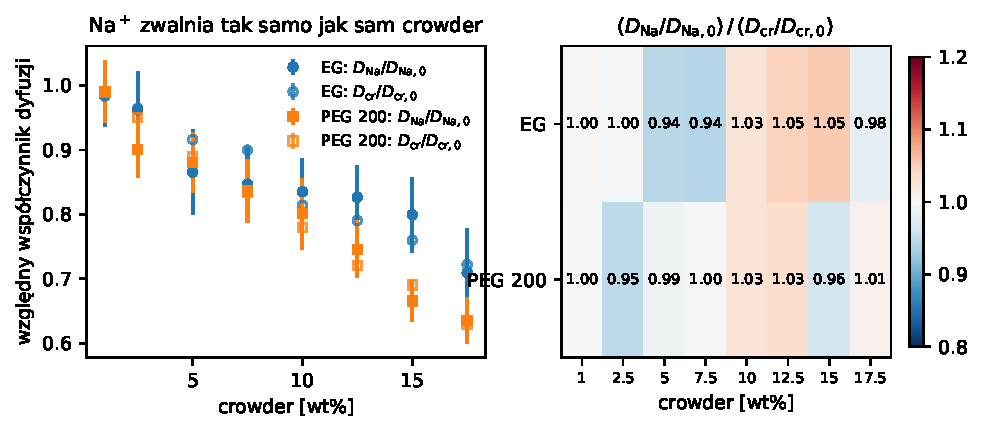
\includegraphics[width=0.95\linewidth]{figures/t1_dosy_ratios.pdf}
\caption{Względne spowolnienie Na$^+$ i samego crowdera. Mapa po prawej: stosunek obu wielkości; 1 oznacza, że Na$^+$ zwalnia dokładnie tak jak niewiążący crowder.}
\end{figure}

\textbf{Wynik.}
\begin{itemize}\itemsep1pt
\item Stosunek spowolnień (średnia ważona): EG $\NratioMeanEG\pm\NratioMeanEGErr$ (zakres $\NratioMinEG$--$\NratioMaxEG$), PEG 200 $\NratioMeanPEGtwo\pm\NratioMeanPEGtwoErr$ (zakres $\NratioMinPEGtwo$--$\NratioMaxPEGtwo$).
\item $\beta n_\mathrm{EG}=\NbnSelfEG\pm\NbnSelfEGErr$~M$^{-1}$ i $\beta n_\mathrm{PEG\,200}=\NbnSelfPEGtwo\pm\NbnSelfPEGtwoErr$~M$^{-1}$. Górne granice $2\sigma$: $\NbnUpperEG$ i $\NbnUpperPEGtwo$~M$^{-1}$. Ekstrapolacja kwadratowa $D_\mathrm{cr,0}$ daje $\NbnSelfQuadEG$ i $\NbnSelfQuadPEGtwo$. Dla porównania wartości z poprawką nanolepkości (Tabela S5 manuskryptu): $\NbnCodeEG\pm\NbnCodeEGErr$ i $\NbnCodePEGtwo\pm\NbnCodePEGtwoErr$~M$^{-1}$.
\end{itemize}

\textbf{Ile wiązania potrzeba, żeby kanałem solnym wyjaśnić EG przy 40~wt\%?} Obserwowane $\dG=\NddGEGforty\pm\NddGEGfortyErr$~kJ/mol przy $c_\mathrm{EG}=\NcEGforty$~M. Wersja spójna (sekcja~3) i wersja manuskryptu:
\begin{equation}
\Delta\ln K=-\frac{\mathrm{SK}}{2}\ln(1+\beta n\,c)\quad\text{(spójna)},\qquad
\Delta\ln K=-\mathrm{SK}\,\ln(1+\beta n\,c)\quad\text{(manuskrypt)}.
\end{equation}
Bez linearyzacji: z krzywej kalibracyjnej $c_\mathrm{eq}=\NcEqEG$~mM daje to samo $\dG$; wtedy $1+\beta n c=(c_0/c_\mathrm{eq})^2$ (spójna) albo $c_0/c_\mathrm{eq}$ (manuskrypt).

\begin{center}
\begin{tabular}{lcccc}
\toprule
wariant & $1+\beta n c$ & związane Na$^+$ & wymagane $\beta n$ [M$^{-1}$] & wymagany sygnał ISE \\
\midrule
manuskrypt, pełna krzywa & $\NreqFullManFactor$ & $\NreqFullManFrac$\% & $\NreqFullManBn$ & $\NreqFullManmV$ mV \\
spójna, pełna krzywa & $\NreqFullConsFactor$ & $\NreqFullConsFrac$\% & $\NreqFullConsBn$ & $\NreqFullConsmV$ mV \\
manuskrypt, liniowo (SK) & $\NreqLinManFactor$ & $\NreqLinManFrac$\% & $\NreqLinManBn$ & $\NreqLinManmV$ mV \\
spójna, liniowo (SK) & $\NreqLinConsFactor$ & $\NreqLinConsFrac$\% & $\NreqLinConsBn$ & $\NreqLinConsmV$ mV \\
\bottomrule
\end{tabular}
\end{center}
Sygnał ISE: $59.16\log_{10}(1+\beta n c)$~mV (spadek wolnego Na$^+$; nachylenie zmierzone przez Bielca: $\NiseSlopeBuf$--$\NiseSlopeEG$~mV/dek.).

\begin{figure}[h]
\centering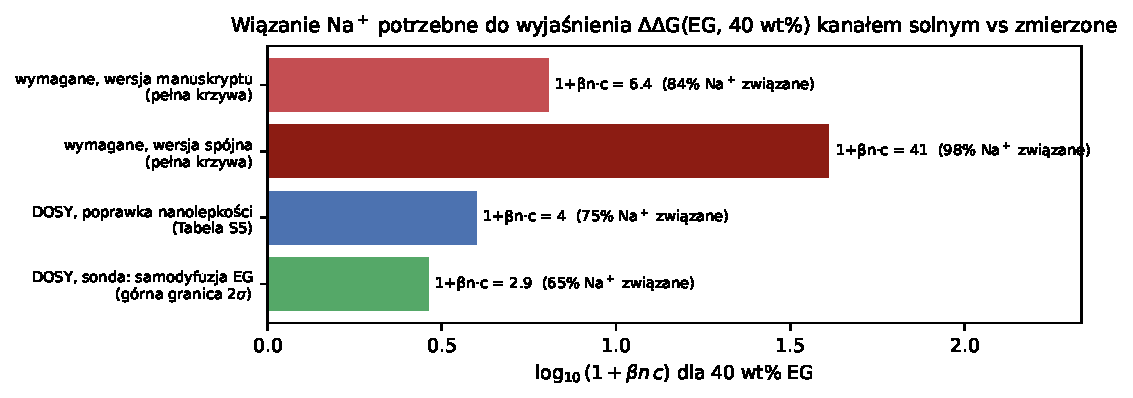
\includegraphics[width=0.92\linewidth]{figures/t1_required_binding.pdf}
\caption{Wiązanie potrzebne do wyjaśnienia destabilizacji EG kanałem solnym (czerwone) vs wiązanie zmierzone DOSY (niebieskie: poprawka nanolepkości; zielone: sonda z samodyfuzji EG, górna granica $2\sigma$).}
\end{figure}

W wersji spójnej nawet wartość z Tabeli S5 ($\beta n=\NbnCodeEG$) wyjaśnia $\NegExplCode$~kJ/mol, czyli $\NegExplFracCode$\% obserwowanego efektu. Górna granica z samodyfuzji daje $\NegExplUpper$~kJ/mol ($\NegExplFracUpper$\%), a globalne $\kappa_\mathrm{EO}=\NkappaCode$ daje $\NegExplKappa$~kJ/mol ($\NegExplFracKappa$\%).

\textbf{Dane niezależne.}
\begin{itemize}\itemsep1pt
\item Bielec 2022, SI sekcja 7: dla glicerolu (który, jak EG, nie brudzi elektrody) różnica między kalibracjami ISE w buforze i w 40~wt\% wynosi około $\NISEglycerol$~mV, tyle samo co zmiana glicerolu 1$\to$40~wt\% bez Na$^+$. Dla EG zakres liniowy i czułość ($\NiseSlopeEG$ mV/dek.) nie zmieniają się względem buforu. Wymagane byłoby $\NreqFullManmV$--$\NreqFullConsmV$~mV.
\item Knowles 2011, SI Tabela S3 (VPO, poliole z KCl jako naśladowcy grup końcowych PEG): sorbitol $\NknMuSorb\pm\NknMuSorbErr$, mannitol $\NknMuMann\pm\NknMuMannErr$, ksylitol $\NknMuXyl\pm\NknMuXylErr$ kcal/molal, czyli zero.
\end{itemize}

\verdict{green}{\textbf{potwierdzona}. Dla EG wiązanie Na$^+$ jest zgodne z zerem. Nawet najhojniejsza wartość z DOSY wyjaśnia najwyżej $\NegExplFracCode$\% destabilizacji EG, a sygnał ISE byłby kilkakrotnie większy niż obserwowany. Dla PEG 200 wynik ten sam, ale z zastrzeżeniem: cząsteczka PEG 200 ($R_h\approx0.30$~nm) jest większa od Na$^+$, więc jej samodyfuzja może przeszacowywać tarcie, a tym samym zaniżać $\beta n$. \textit{Co by rozstrzygnęło:} $^{31}$P DOSY fosforanu albo $D$ wody (HDO) w tych samych próbkach jako sonda niewiążąca innej wielkości oraz VPO/krioskopia EG + NaPi.}

\section{Teza 2: człon elektrostatyczny jest przeszacowany i może mieć zły znak}

\textbf{Rama.} Hybrydyzacja nie zmienia ładunku DNA, więc $\Delta\Gamma_+=\Delta\Gamma_-$, a DNA reaguje tylko na iloczyn $a_+a_-$:
\begin{equation}
d\ln K=\mathrm{SK}\;d\ln\apm,\qquad
\left(\frac{\partial\ln K}{\partial x}\right)_{\!s}=\left(\frac{\partial\ln K}{\partial x}\right)_{\!\apm}+\frac{\mathrm{SK}}{2RT}\,\mu_x,\qquad \mu_x\equiv\left(\frac{\partial\mu_\mathrm{s\acute{o}l}}{\partial x}\right)_{\!s}.
\end{equation}
Jeśli PEG wiąże tylko kation, to $a_+\propto c_\mathrm{eff}=c_0/(1+\beta n c)$ i $a_-\propto c_0$, więc z krzywej buforowej trzeba odczytać
\begin{equation}
c_\mathrm{eq}=\sqrt{c_\mathrm{eff}\,c_0}=\frac{c_0}{\sqrt{1+\beta n\,c_\mathrm{PEG}}},\qquad \Delta\Delta G_\mathrm{el}=\Delta G_\mathrm{hyb}(c_\mathrm{eq})-\Delta G_\mathrm{hyb}(c_0).
\end{equation}
„Rozcieńczenie” $c_0$ ($35\to22.5$~mM przy 40~wt\%) jest artefaktem skali molowej, bo molalność soli jest stała. Warianty: (a) obecny kod (sprawdzone: odtwarza \texttt{dG\_Na} z pipeline); (b) bez rozcieńczenia, $c_\mathrm{eff}$; (c) $c_\mathrm{eq}$, $\kappa_\mathrm{EO}=\NkappaCode$; (d) $c_\mathrm{eq}$, $\kappa_\mathrm{EO}=0.088$ i $0.055$ (alternatywne poprawki lepkościowe, recenzja M2); (e) netto jak PEG--KCl u Knowlesa:
\begin{equation}
\Delta\Delta G_\mathrm{s\acute{o}l}=-\frac{\mathrm{SK}}{2(1+\varepsilon)}\,\mu_x\,x,\qquad \mu_x=+\NMUXKCL~\mathrm{kcal\,(mol\cdot molal\ mon.)^{-1}},\quad 1+\varepsilon=\NonePlusEps.
\end{equation}

\begin{figure}[h]
\centering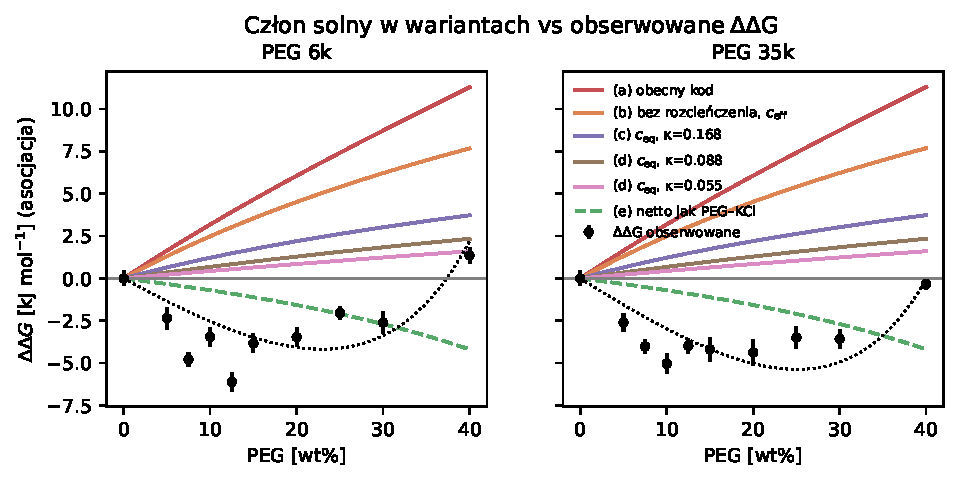
\includegraphics[width=0.95\linewidth]{figures/t2_variants.pdf}
\caption{Człon solny w wariantach (a)--(e) i obserwowane $\dG$ (punkty; kropkowana linia: dopasowanie kwadratowe w $x$).}
\end{figure}

\textbf{Przy 40~wt\% PEG 35k} ($\dG_\mathrm{obs}=\NddGobsFortyPEGthirtyfive$~kJ/mol): (a) $\Natfourzeroa$, (b) $\Natfourzerob$, (c) $\Natfourzeroc$, (d) $\Natfourzerodone$ / $\Natfourzerodtwo$, (e) $\Natfourzeroe$~kJ/mol.

\textbf{Ułamek wahnięcia.} Wahnięcie to $\dG(40\%)-\dG(x_\mathrm{min})$ z gładkiego dopasowania; dla długich PEG wynosi od $\NswingPEGthreek\pm\NswingPEGthreekErr$ (PEG 3k) do $\NswingPEGonek\pm\NswingPEGonekErr$~kJ/mol (PEG 1k). Wyjaśniany ułamek (średnio, zakres po PEG): (a) $\NfracMeana$\% ($\NfracMina$--$\NfracMaxa$), (b) $\NfracMeanb$\%, (c) $\NfracMeanc$\% ($\NfracMinc$--$\NfracMaxc$), (d) $\NfracMeandone$\% i $\NfracMeandtwo$\%, (e) $\NfracMeane$\% (przeciwny kierunek).

\begin{figure}[h]
\centering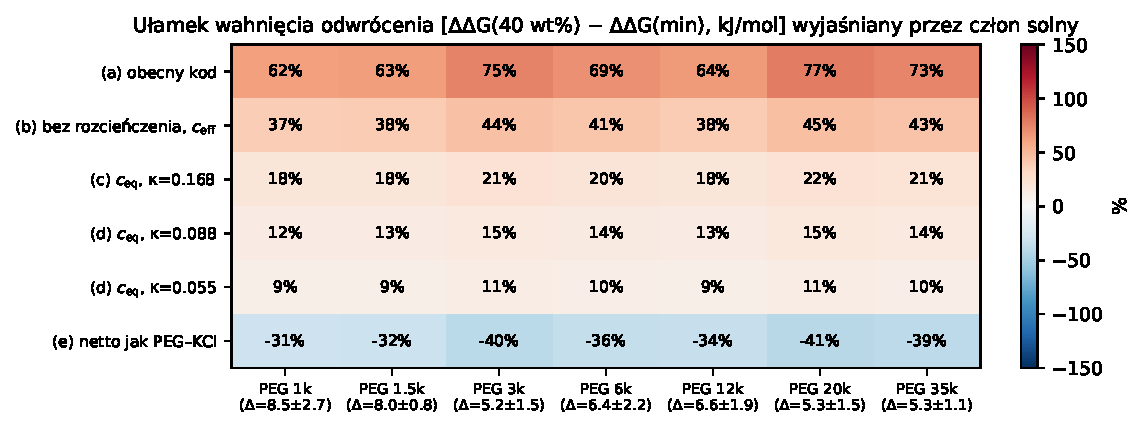
\includegraphics[width=0.92\linewidth]{figures/t2_fraction_heatmap.pdf}
\caption{Ułamek wahnięcia odwrócenia wyjaśniany przez każdy wariant członu solnego, dla każdego długiego PEG.}
\end{figure}

\textbf{Krzywizna.} Współczynnik kwadratowy (zerowy wyraz wolny, PEG 35k): obserwowane $\Ncurvobs\pm\NcurvObsSigma$~J\,mol$^{-1}$/molal$^2$ (wypukłe), człon solny (a) $\Ncurva$, (b) $\Ncurvb$, (c) $\Ncurvc$ (wklęsłe). Wiązanie daje $\ln(1+\beta n c)$, czyli destabilizację najsilniejszą na początku i słabnącą. Odwrócenie wymaga członu narastającego. \textbf{Kanał solny w żadnym wariancie nie może sam wytworzyć minimum;} w manuskrypcie robi to dopiero malejące $V_\mathrm{eff}$ w residuum.

\textbf{Degeneracja testu „dosypanie soli przywraca $K$”.} Dla kalibracji potęgowej (Bielec 2022: $K=Xc^{Y}$, $Y=2.51$):
\begin{equation}
K\!\left(\tfrac{c}{f}\right)=X c^{Y} f^{-Y}=K(c)\cdot f^{-Y}
\quad\Longrightarrow\quad
\underbrace{c\to c/f}_{\text{wiązanie}}\ \equiv\ \underbrace{\dG=Y\,RT\ln f}_{\text{stała kara}}.
\end{equation}
Z takich danych $\kappa$ wyjdzie stałe niezależnie od mechanizmu. Rozróżnienie jest możliwe tylko tam, gdzie SK$(c)$ się zmienia. Z kalibracji SK$(c_0)=\NSKmodel$, a SK$(150~\mathrm{mM})=\NSKhighc$. Dane z SI (Tab.~S3, $\NnSIbeyond$ punktów powyżej 175~mM, poza kalibracją) pokazują maksimum $K$ przy około 175~mM. Wiązanie przewiduje maksimum tej samej wysokości przy wyższym $c$; mechanizm nieelektrostatyczny przewiduje niższe maksimum przy tym samym $c$.

\begin{figure}[h]
\centering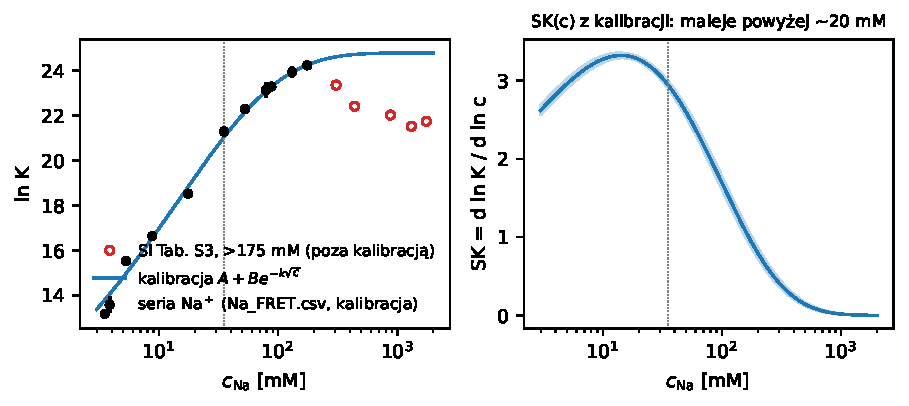
\includegraphics[width=0.85\linewidth]{figures/t2_SK.pdf}
\caption{Seria solna i SK$(c)$. Odróżnienie przesunięcia poziomego od pionowego wymaga pomiaru przez maksimum $K(c)$.}
\end{figure}

\verdict{green}{\textbf{potwierdzona w części „przeszacowany”}: poprawienie dwóch błędów formalnych (pierwiastek, rozcieńczenie) zmniejsza wkład z $\NfracMeana$\% do $\NfracMeanc$\% wahnięcia, a krzywizna członu solnego jest przeciwna do obserwowanej. \textbf{Nierozstrzygnięta w części „zły znak”}: jedyny pomiar netto ($\mu_x>0$) dotyczy PEG--KCl, a nie PEG--NaPi. \textit{Co by rozstrzygnęło:} VPO/krioskopia $\mu_x$ dla PEG + NaPi; seria $K(c_\mathrm{Na})$ przez maksimum w 2--3 roztworach crowdera.}

\section{Teza 3: rama Knowlesa}

\textbf{m-wartości na monomer} (liniowo, $0<x\le5.5$, kcal\,mol$^{-1}$/molal mon., znak asocjacji): EG $\NmEG\pm\NmEGErr$; PEG 200 $\NmPEGtwozerozero\pm\NmPEGtwozerozeroErr$ (w pełnym zakresie $\NmPEGtwoFull\pm\NmPEGtwoFullErr$); PEG 400 $\NmPEGfourzerozero\pm\NmPEGfourzerozeroErr$; PEG 600 $\NmPEGsixzerozero\pm\NmPEGsixzerozeroErr$; PEG 1k--35k od $\NmPEGonepfivek$ do $\NmPEGthreek$ (typowo $\pm0.17$). Knowles (znak odwrócony do asocjacji): EG $+\NknEG$, PEG 200 $+\NknPEGtwo$, PEG 600 lekka stabilizacja, plateau $\NknHigh\pm\NknHighErr$ (liniowo) / $\NknHighQuad$ (kwadratowo). \textbf{Minimum} $\dG$ dla PEG $\geq$1k: $x_\mathrm{min}=\NxminPEGonek$--$\NxminPEGthreefivek$ monomolal ($\NwtminPEGonek$--$\NwtminPEGthreefivek$~wt\%); u Knowlesa $\approx\NknXrev$, niezależnie od $M$.

\begin{figure}[h]
\centering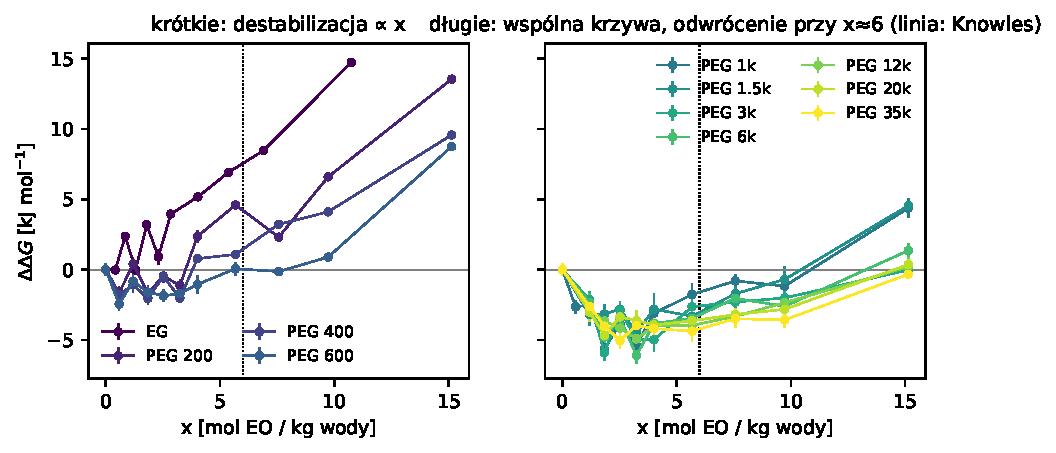
\includegraphics[width=0.95\linewidth]{figures/t3_monomolal.pdf}
\caption{$\dG$ na skali molalności monomeru. Kropkowana linia: położenie odwrócenia u Knowlesa.}
\end{figure}

\textbf{Model zerowy na monomer} (konwencja asocjacji, $s(N)=1/[1+(N/N_{1/2})^2]$):
\begin{equation}
\frac{m}{N}=-\Big\{\big[\chi_\infty+(1-\chi_\infty)\,s(N)\big]\,P+E_\infty\,\big[1-s(N)\big]\Big\},\qquad P=\alpha_I\,\mathrm{ASA}_I\,\Delta\mathrm{ASA},
\end{equation}
gdzie $P$ to człon preferencyjnych oddziaływań przy pełnej dostępności, a $E_\infty$ to objętość wyłączona Hermansa na monomer. Parametry Knowlesa przeskalowane na 13 bp ($\Delta$ASA$\times13/12$) i 298~K: $-P=\NPKnowles$, $-E_\infty=\NEKnowles$, plateau $\NplateauKnowlesPred$ (zgodność bez dopasowania: $\chi^2/N=\NpredChi$). Dopasowanie ($\chi_\infty=\NknChiInf$ stałe): $-P=\NnullP\pm\NnullPErr$, $-E_\infty=\NnullE\pm\NnullEErr$, $N_{1/2}=\NnullNh\pm\NnullNhErr$, maksymalna reszta $\NnullMaxRes\sigma$ ($\chi^2_\mathrm{red}=\NnullChi$; test słaby, bo błędy m-wartości są zdominowane przez wspólny błąd $K_0$).

\begin{figure}[h]
\centering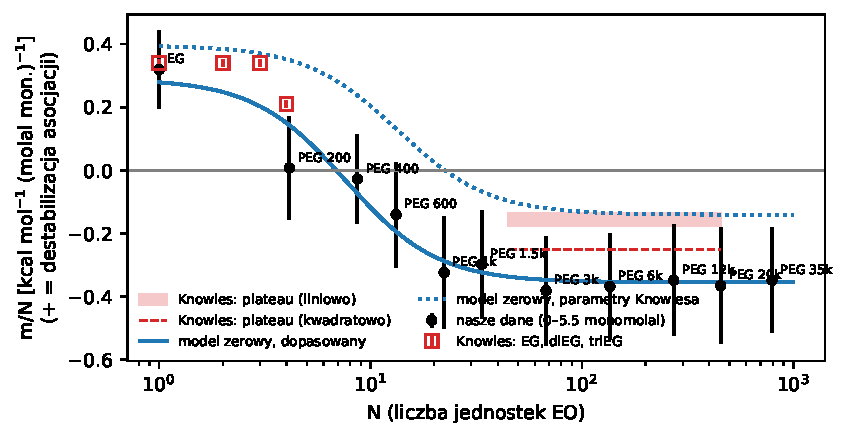
\includegraphics[width=0.82\linewidth]{figures/t3_mN.pdf}
\caption{m-wartości na monomer vs $N$: nasze dane, Knowles i model zerowy.}
\end{figure}

\textbf{Czy reszta wymaga Na$^+$?} Stały człon solny na monomer dla długich PEG jest zdegenerowany z $E_\infty$. Dlatego ustaliłem $E_\infty$ na wartości Knowlesa i dopasowałem dodatkowy człon $S\,[1-s(N)]$: $S=\NsaltS\pm\NsaltSErr$ kcal/(mol·molal mon.). DOSY w wersji spójnej przewiduje $S=+\frac{\mathrm{SK}}{2(1+\varepsilon)}RT\,\kappa_\mathrm{EO}=\NSdosyA$ ($\kappa=0.168$), $\NSdosyB$ (0.088) albo $\NSdosyC$ (0.055). Dopasowanie ma \emph{przeciwny znak}, czyli dane chcą więcej stabilizacji niż EV Knowlesa, a nie destabilizacji od Na$^+$. Wynik zależy jednak od przeskalowania EV.

\textbf{Obraz odwrócenia.} Dopasowanie z załamaniem ($s_1$ poniżej, $s_2$ powyżej $x^*$):
\begin{equation}
\dG(x)=s_1x+(s_2-s_1)\,w\ln\!\big(1+e^{(x-x^*)/w}\big)\ \ (\text{minus wartość w }x=0),\quad w=1.
\end{equation}
Przy $x^*=\NknXrev$ (Knowles): $s_1=\NbroSixSone\pm\NbroSixSoneErr$ (Knowles: $\NknHighQuad$), $s_2=\NbroSixStwo\pm\NbroSixStwoErr$, a PEG 200 daje $\NmPEGtwoFull\pm\NmPEGtwoFullErr$. Zgodność z obrazem „po odwróceniu PEG zachowuje się jak PEG 200” jest bardzo dobra. Przy swobodnym $x^*$ dopasowanie jest jednak dużo lepsze ($\chi^2$: $\NchiFreeTot$ vs $\NchiSixTot$ dla $x^*=6$ i $\NchiQuadTot$ dla paraboli; $\NnBroTot$ punktów), z $x^*$ między $\NbroXsMin$ a $\NbroXsMax$ i $s_2=\NbroStwo\pm\NbroStwoErr$. Nasza stabilizacja nasyca się wcześnie (około 5~wt\%) zamiast rosnąć liniowo do 6 monomolal. Może to być realna różnica (inna sól, $T$) albo artefakt sufitu oznaczalności $K\sim10^{10}$ przy 10~nM donora (recenzja M7).

\begin{figure}[h]
\centering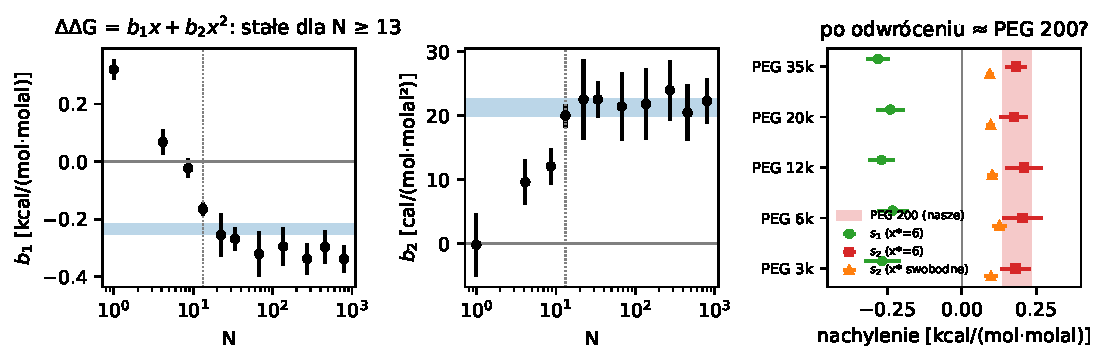
\includegraphics[width=0.95\linewidth]{figures/t3_coeffs_broken.pdf}
\caption{Lewo i środek: współczynniki $\dG=b_1x+b_2x^2$ vs $N$ (pasmo: średnia ważona dla $N\geq13$). Prawo: nachylenia przed i po odwróceniu vs nachylenie PEG 200.}
\end{figure}

\textbf{Niezależność od $M$ powyżej około 600~Da.} Dla PEG $\geq600$: $b_2=\NbTwoMean\pm\NbTwoMeanErr$~cal/(mol·molal$^2$), CV $\NbTwoCV$\%, $\chi^2_\mathrm{red}=\NbTwoChi$; $b_1=\NbOneMean\pm\NbOneMeanErr$, CV $\NbOneCV$\% ($\NbOneCVOnek$\% dla $\geq$1k). Rozrzut gładkich krzywych przy 20~wt\% wynosi $\NspreadTwenty$~kJ/mol przy średniej $\NmeanTwenty$~kJ/mol. Test F wspólnej krzywej: PEG $\geq600$ $F=\NFstat$ ($p<0.01$), PEG $\geq$1k $F=\NFstatOnek$ ($p=\NFpvalOnek$). Odpowiedź jest więc w przybliżeniu niezależna od $M$ (do około 1~kJ/mol), ale statystycznie nie identyczna.

\verdict{orange}{\textbf{częściowo potwierdzona}. Na skali monomeru nasze dane odtwarzają Knowlesa ilościowo: m-wartość EG, plateau długich PEG, położenie minimum, nachylenie po odwróceniu równe PEG 200. Model zerowy nie potrzebuje Na$^+$, a człon solny dopasowuje się ze znakiem przeciwnym do przewidywanego z DOSY. Różnice: EV około $1.5\times$ większe niż u Knowlesa i wcześniejsze nasycenie stabilizacji. \textit{Co by rozstrzygnęło:} $K$ przy 1~nM donora w gałęzi stabilizacji (czy nasycenie jest realne); $\mu_x$ dla PEG + NaPi; 1--2 punkty przy innej soli.}

\section{Teza 4: minimal viable paper bez nowych eksperymentów (A0)}

\textbf{Collapse $V_\mathrm{eff}$.} Odtworzyłem obliczenie z \texttt{figures\_publication.ipynb} (komórka 8) i porównałem z wersją, w której residuum zastąpiono stałą. Residuum z danych: nachylenie $\NcollrealAlpha$, $R^2=\NcollrealRtwo$. Stała dla każdego PEG: $\NcollconstPEGAlpha$, $R^2=\NcollconstPEGRtwo$. Jedna stała dla wszystkich: $\NcollconstAllAlpha$, $R^2=\NcollconstAllRtwo$. Residuum ma średnią $\NrestMean$ i odchylenie $\NrestSD$~kJ/mol. \textbf{Prawie cała jakość collapse'u jest algebraiczna}, więc Fig.~4e--f należy usunąć.

\begin{figure}[h]
\centering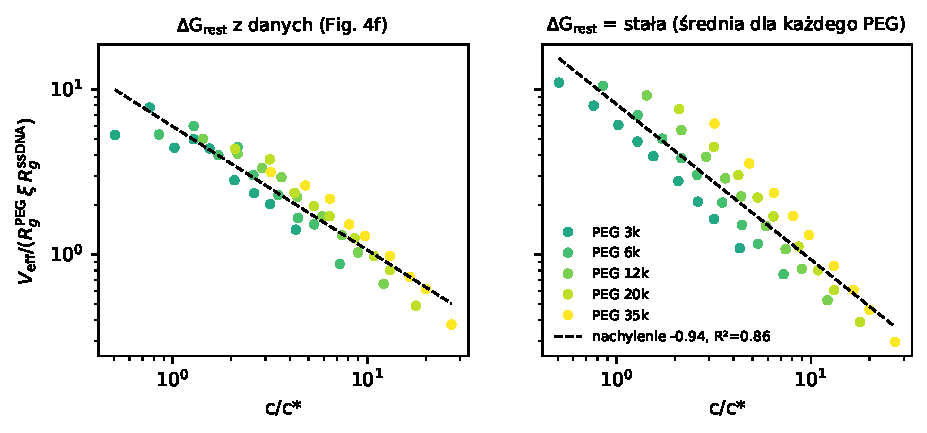
\includegraphics[width=0.85\linewidth]{figures/t4_collapse.pdf}
\caption{Collapse z Fig.~4f (lewo) i ten sam rachunek ze stałym residuum (prawo).}
\end{figure}

\textbf{Tytuł roboczy.} \emph{Polymer length and monomer concentration, not ion sequestration, set the crossover from stabilization to destabilization of DNA duplexes in PEG solutions.}

\textbf{Abstrakt (szkic).} We measured the equilibrium constant of 13-bp DNA hybridization by FCS in ethylene glycol and ten PEGs (200--35\,000~Da) up to 40~wt\%. On a monomer-molality scale, short glycols destabilize the duplex with a per-monomer m-value matching preferential-interaction estimates, whereas PEGs above about 600~Da stabilize it with a molecular-weight-independent per-monomer effect and reverse at a common monomer concentration of about 6--7~mol/kg, irrespective of the overlap concentration. Diffusion NMR shows that Na$^+$ is not bound by ethylene glycol or PEG 200 but is weakly associated with longer chains. A thermodynamically consistent linkage analysis shows that this association can account for at most about one fifth of the reversal and has the wrong curvature to produce it. The data are quantitatively consistent with a two-term description (preferential interactions with exposed bases plus excluded volume, with segment accessibility rising in the entangled regime), extending Knowles et al.\ to lower salt, Na$^+$, 25~°C and higher molecular weights.

\textbf{Rysunki (jeden przekaz na rysunek).}
\begin{enumerate}\itemsep1pt
\item $K$ i $\dG$ vs wt\% dla 11 crowderów: przejście od monotonicznej destabilizacji do odpowiedzi dwufazowej.
\item Te same dane na skali monomolalnej: krzywe długich PEG się nakładają, minimum przy stałym $x$.
\item m-wartości na monomer vs $N$ z Knowlesem i modelem zerowym: jedna rama opisuje cały szereg.
\item DOSY: Na$^+$ nie wiąże się z EG i PEG 200, słabo z długimi PEG (próg długości łańcucha).
\item Bilans kanału solnego: warianty (a)--(e) i krzywizna; elektrostatyka nie tworzy odwrócenia.
\end{enumerate}
\textbf{Do SI:} szczegóły DOSY z trzema poprawkami lepkościowymi; seria solna i SK$(c)$; dopasowania z załamaniem; wrażliwość na V$_\mathrm{ef}$ i RI; tabele.

\textbf{Do usunięcia lub osłabienia:} „electrostatic repulsion” w tytule; c$_\mathrm{Na,eff}=c_0/(1+\beta n c)$ i „rozcieńczenie” $c_0$; interpretacja residuum wyłącznie jako deplecji; collapse $V_\mathrm{eff}$ (Fig.~4e--f); trend $a_1,a_2$ vs DP w jednostkach molowych (Fig.~2e--f); zdanie, że Na$^+$ wyjaśnia destabilizację krótkich crowderów.

\textbf{Ryzyka recenzenckie i odpowiedzi bez nowych pomiarów.}
\begin{itemize}\itemsep1pt
\item \emph{Brak $\mu_x$ dla PEG + NaPi.} Pokazać wynik jako przedział od (c) do (e) i zaznaczyć, że wniosek „Na$^+$ nie tworzy odwrócenia” nie zależy od znaku (krzywizna).
\item \emph{Kalibracja V$_\mathrm{ef}$ (0.18--0.42 fl) i ciasne wiązanie.} Analiza wrażliwości ($\chi/\chi(0)$, $V=\mathrm{const}$, $V\propto\mathrm{RI}$), propagacja niepewności V$_\mathrm{ef}$; wnioski oprzeć na nachyleniach i położeniu minimum, a nie na absolutnym $K\sim10^{10}$.
\item \emph{Pokrycie z Knowlesem 2011.} Zaprezentować jako niezależne potwierdzenie przy innej soli, kationie, $T$ i metodzie, rozszerzone do 35k.
\item \emph{Sprzeczność z Bielec 2022.} Omówić jawnie: przywracanie $K$ solą jest zdegenerowane (sekcja 3), a ISE nie potwierdza wiązania przez EG i glicerol.
\item \emph{Para FRET} (Bielec 2022: $K$ około 3$\times$ wyższe niż para z jednym znacznikiem). Zdanie o możliwej zależności stackingu barwników od crowdera.
\end{itemize}

\textbf{Trzy najtańsze eksperymenty o największym zysku.}
\begin{enumerate}\itemsep1pt
\item \textbf{Krioskopia lub VPO dla PEG + NaPi} (2--3 masy PEG, 2--3 stężenia soli): bezpośrednio $\mu_x$, czyli znak i wielkość kanału solnego.
\item \textbf{Dializa równowagowa} NaPi przez membranę zatrzymującą PEG 6k--35k: współczynnik $\Gamma$ sól--PEG (rozdział kation/anion, oznaczenie Na$^+$ i fosforanu).
\item \textbf{Seria $K(c_\mathrm{Na})$ przez maksimum (10--400 mM) w 30~wt\% EG}: przesunięcie poziome vs pionowe rozstrzyga mechanizm bez żadnego modelu.
\end{enumerate}

\section{Założenia i rzeczy, których nie udało się sprawdzić}
\begin{itemize}\itemsep1pt
\item Samodyfuzja crowdera jako miara tarcia w skali Na$^+$: ścisłe dla EG (podobny rozmiar), przybliżone dla PEG 200; dla PEG $\geq$400 nieużyteczne.
\item Model szybkiej wymiany, stężenia molowe łańcuchów jak w kodzie, $D_\mathrm{cr,0}$ z ekstrapolacji liniowej (kwadratowa: wynik bez zmian jakościowych).
\item Kalibracja solna dotyczy tylko $c\leq175$~mM (\texttt{Na\_FRET.csv}). Punkty powyżej pochodzą z tabeli w SI manuskryptu i nie są w danych repozytorium.
\item SK: lokalne nachylenie z danych ($\NSKlocal$) różni się od pochodnej modelu kalibracji ($\NSKmodel$); warianty pełnej krzywej używają modelu.
\item $(1+\varepsilon)=\NonePlusEps$ z przybliżenia Daviesa dla soli 1:1 przy 0.035~m; fosforan jest mieszaniną 1:1/2:1.
\item Wariant (e) to $\mu_x$ dla PEG--KCl (VPO, PEG 1000/2000, 25~°C), zastosowane liniowo do 40~wt\%. \textbf{$\mu_x$ dla PEG + NaPi nie jest znane.}
\item Parametry Knowlesa przeskalowane na 13 bp liniowo z $\Delta$ASA (EV też liniowo z długością) i na 298~K przez $RT$; $\chi_\infty$ przyjęte, a $s(N)$ sigmoidalne z $h=2$.
\item Błędy $K$ są zaniżone ($\chi^2_\mathrm{red}\sim10$); m-wartości zdominowane przez wspólny błąd $K_0$; testy $\chi^2$ modelu zerowego są przez to słabe.
\item Nie sprawdzono: wpływu stałej dielektrycznej, zależności stackingu barwników od crowdera, wyników przy 1~nM donora ani kalibracji V$_\mathrm{ef}$ in situ.
\end{itemize}

\end{document}
